\chapter{Integração}

Nos capítulos anteriores foi apresentado o detalhe de cada subsistema do projeto, neste será detalhado o processo de integração de cada subsistema.

\section{Software - Eletrônica}

Sendo a principal interface entre o usuário da bancada e o motor o SBAM possui a seguinte interface inicial.
Onde o usuário deverá fazer um login antes de iniciar a	 análise. 

\begin{figure}[h!]
	\centering
	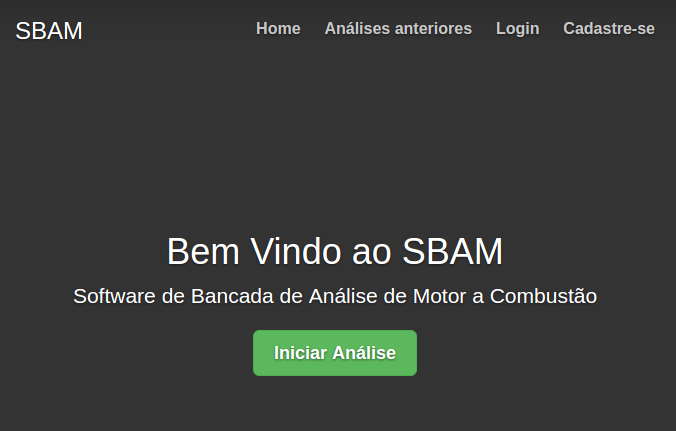
\includegraphics[keepaspectratio=true,scale= 0.7]{figuras/SBTM-TelaInicial.png}
	\caption{Tela inicial SBTM}
	\label{telainicialSbtm}
\end{figure}

Após a realização da autenticação pode-se realizar o acionamento do motor e o usuário da bancada é redirecionado para a tela da da figura \ref{acionamentoDoMotor}, o detalhamento do processo de integração da parte de controle é apresentado nas subseções seguintes.

\subsection{Controle}

Para realização do módulo de controle o usuário deverá acionar o motor, selecionando o botão apresentado na figura \ref{acionamentoDoMotor}. 

\begin{figure}[h!]
	\centering
	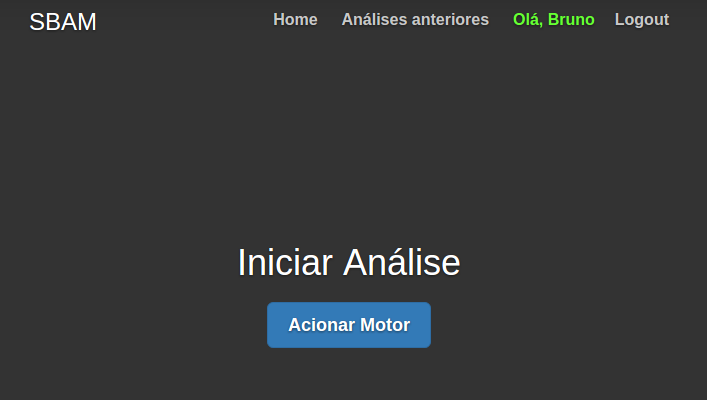
\includegraphics[keepaspectratio=true,scale= 0.7]{figuras/acionarMotor.png}
	\caption{Tela de acionamento do motor}
	\label{acionamentoDoMotor}
\end{figure}
  


\subsection{Aquisição}